\documentclass[11pt,a4paper]{article}
\usepackage[T1]{fontenc}
\usepackage[margin=2.3cm]{geometry}
\usepackage{amsmath,amssymb}
\usepackage{graphicx}
\usepackage[dvipsnames]{xcolor}
\usepackage{enumitem}
\usepackage[colorlinks=true,linkcolor=blue,urlcolor=blue]{hyperref}
\setlength{\parskip}{0.6em}
\setlength{\parindent}{0pt}
\begin{document}

\begin{center}{\LARGE\bfseries openevacuation}\\[0.4em]{\large Plan a safe evacuation from a building with crowd flow, in three sessions.}\\[0.2em]\small PAN IIT OSS explainer \textbullet{} higher secondary to diploma / undergraduate (levels 4-5)\end{center}

\section*{Why this exists}
People move like a flow, and exits and corridors set how quickly a building can be emptied. This explainer follows the idea from a crowd passing one door to the speed-density law of real crowds, bottlenecks and queues, and a validated simulation of a multi-storey building, using only arithmetic, a straight line and a parabola.

\section*{The end goal}
Plan a safe evacuation from a building with crowd flow: find where the queues form, estimate the required safe escape time (RSET), compare it with the available safe escape time (ASET) with a safety margin, and choose the number and width of stairs so that the plan still works when one route is blocked. \textbf{Safety:} these are simplified educational models, not design tools. Real buildings must follow the fire code (in India, the National Building Code, Part 4: Fire and Life Safety) and be checked by a qualified fire engineer.

\section*{How the three sessions build up}
\begin{enumerate}[nosep]
\item \textbf{Session 1: People flow through a door} (Level 1, conceptual interactive model, 60 min).
\item \textbf{Session 2: Speed, density and the bottleneck} (Level 2, mathematical engineering model, 75 min).
\item \textbf{Session 3: Simulate a building evacuation and plan it safely} (Level 3, simulation and validation, 90 min).
\end{enumerate}

\section{Session 1: People flow through a door}

\subsection*{A. Real-world problem}
A fire alarm rings during a college function. 240 people are in the hall and there is one 1.2 m exit door, 20 m from the middle of the hall. How long until the last person is outside? Would a second door halve that time? Fire engineers answer this with a surprisingly simple idea: a crowd moving through a door behaves like water flowing through a pipe, and the narrowest part sets the pace. (General education only: this is a simplified model, not a building design method.)

\subsection*{B. Concept and theory}
Stand next to a door and count the people who pass each second: that number is the \textbf{flow} F. It depends on how tightly packed the crowd is (the density D, persons per square metre), how fast it moves (v, m/s) and how wide the passage is (W, m): F = D v W. In a dense moving crowd of about 2 persons/m2 people shuffle at about 0.65 m/s, so each metre of width passes about 1.3 persons per second. This number, the \textbf{specific flow} Fs, makes hand calculations possible. People keep a small gap from the door frame, so only the \textbf{effective width} We = clear width - 2 x 0.15 m is used; a 1.2 m door is effectively 0.9 m wide and passes Fs We = 1.17 persons/s. The time to empty a room has three parts: the \textbf{pre-movement time} (hearing the alarm, deciding, picking up a bag), the walk of the first people to the door, and the \textbf{queue time} N / F for N people to pass a door that lets F persons through each second. This is the simplest form of the "hydraulic model" in fire engineering handbooks.

\begin{itemize}[nosep]
\item F: flow: people passing per second (persons/s)
\item D: crowd density (persons/m2)
\item v: walking speed (m/s)
\item W, We: clear width and effective width of the opening (m)
\item Fs: specific flow: flow per metre of effective width (persons/(s m))
\item N: number of people to evacuate (persons)
\item t\_pre: pre-movement time (alarm to starting to move) (s)
\item L: walking distance to the door (m)
\end{itemize}

\begin{equation*}
F = D\,v\,W
\end{equation*}

\begin{equation*}
W_e = W - 2 \times 0.15\ \mathrm{m},\qquad F_{\mathrm{door}} = F_s\,W_e
\end{equation*}

\begin{equation*}
t_{\mathrm{evac}} = t_{\mathrm{pre}} + \frac{L}{v} + \frac{N}{F_{\mathrm{door}}}
\end{equation*}

\begin{center}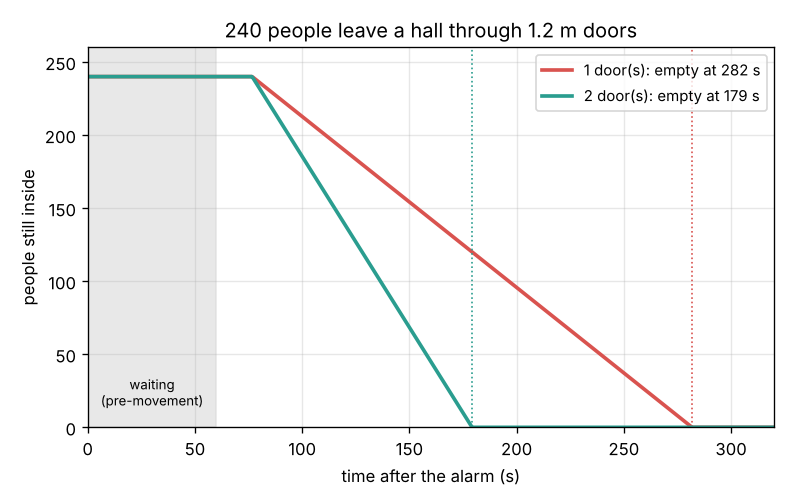
\includegraphics[width=0.85\linewidth]{figures/s01_room_emptying.png}\\\small 240 people leave a hall through one or two 1.2 m doors; the number inside falls at the door flow after the pre-movement time.\end{center}

\subsection*{E. Worked example}
240 people are in a hall with one exit door of clear width 1.2 m. The pre-movement time is 60 s, the walk to the door is 20 m at 1.2 m/s and the specific flow is 1.3 persons/(s m). Find the evacuation time, then repeat with two such doors.
\begin{enumerate}[nosep]
\item Effective width: We = 1.2 - 2 x 0.15 = 0.9 m.
\item Door flow: F = 1.3 x 0.9 = 1.17 persons/s.
\item Walking time: 20 / 1.2 = 16.7 s; queue time: 240 / 1.17 = 205.1 s.
\item One door: t = 60 + 16.7 + 205.1 = 281.8 s, about 4.7 minutes.
\item Two doors: F = 2.34 persons/s, queue time 102.6 s, t = 60 + 16.7 + 102.6 = 179.2 s, about 3.0 minutes.
\end{enumerate}
\textbf{Answer.} 282 s with one door, 179 s with two: the second door saves 103 s, which is only the half of the queue time.

\subsection*{F. Questions}
\begin{enumerate}[nosep]
\item \textbf{Conceptual.} A second identical door is added to the hall. Why does the evacuation time not halve?
\item \textbf{Numerical.} A classroom holds 150 people and has one 1.0 m door 12 m away. The pre-movement time is 30 s and the walking speed 1.2 m/s. Find the evacuation time with Fs = 1.3 persons/(s m). Check the units.
\item \textbf{Graph and simulation interpretation.} In the door-width figure, doubling the clear width of one door from 1.2 m to 2.4 m cuts the queue time by more than half. Why? Find both queue times and both total times.
\item \textbf{Design and optimisation challenge.} Design: a hall for 300 people must be empty within 240 s of the alarm (pre-movement 60 s, walk 20 m at 1.2 m/s). Compare two 1.0 m doors, two 1.2 m doors and one 1.8 m door. Which meet the limit, and which would you choose?
\end{enumerate}

\section{Session 2: Speed, density and the bottleneck}

\subsection*{A. Real-world problem}
Students leave a lecture block along a 2 m wide corridor. Its end is a 1.2 m door into the stair. Will a queue form at that door? How fast will it grow, and what width of door would avoid it? And why do announcements say "do not push"? If everyone squeezes closer, surely more people get through? (Simplified hydraulic model of crowd movement; not a design method.)

\subsection*{B. Concept and theory}
Measurements of real crowds (Fruin, Pauls, Predtechenskii and Milinskii, collected in the SFPE Handbook of Fire Protection Engineering) show that walking speed falls roughly in a straight line as the crowd gets denser: v = k (1 - a D) with a = 0.266 m2/person. On level ground, in corridors and through doors k = 1.40 m/s. In a thin crowd (below about 0.55 persons/m2) people are not slowed by others and walk at a free speed of 0.85 k = 1.19 m/s. At D = 1 / a = 3.8 persons/m2 the crowd is jammed. The specific flow Fs = D v = k D (1 - a D) is a downward parabola: zero when the corridor is empty (no people) and zero when it is jammed (no speed). Its top is half way, at D* = 1 / (2a) = 1.88 persons/m2, where Fs\_max = k / (4a) = 1.32 persons/(s m): the 1.3 of Session 1. Above D* more crowding means less flow. On stairs people step tread by tread, so k is lower and depends on the steps; for the common 178 mm riser and 279 mm tread k = 1.08 m/s (speed along the slope) and Fs\_max = 1.02 persons/(s m). People are neither created nor lost where a corridor meets a door, so the flow in equals the flow out: Fs\_in We\_in = Fs\_out We\_out. If this asks the narrower passage for more than its Fs\_max, it cannot carry it: a queue forms, the passage runs at its maximum flow, and the queue grows at the difference.

\begin{itemize}[nosep]
\item v: walking speed (m/s)
\item D: crowd density (persons/m2)
\item k: speed constant: 1.40 level, 1.00 to 1.23 stairs (m/s)
\item a: slope of the speed-density law, 0.266 (m2/person)
\item Fs: specific flow D v (persons/(s m))
\item D*: density of maximum flow, 1 / (2a) (persons/m2)
\item We: effective width: clear width minus 0.15 m (doors, stairs) or 0.20 m (corridor walls) at each side (m)
\item F: total flow Fs We (persons/s)
\end{itemize}

\begin{equation*}
v = k\,(1 - a D),\qquad a = 0.266\ \mathrm{m^2/person}
\end{equation*}

\begin{equation*}
F_s = D\,v = k D (1 - a D)
\end{equation*}

\begin{equation*}
D^{*} = \frac{1}{2a},\qquad F_{s,\max} = \frac{k}{4a}
\end{equation*}

\begin{equation*}
F_{s,\mathrm{in}}\,W_{e,\mathrm{in}} = F_{s,\mathrm{out}}\,W_{e,\mathrm{out}} \quad\text{(if } F_{s,\mathrm{out}} \le F_{s,\max}\text{, otherwise a queue grows at } F_{\mathrm{in}} - F_{\max})
\end{equation*}

\begin{center}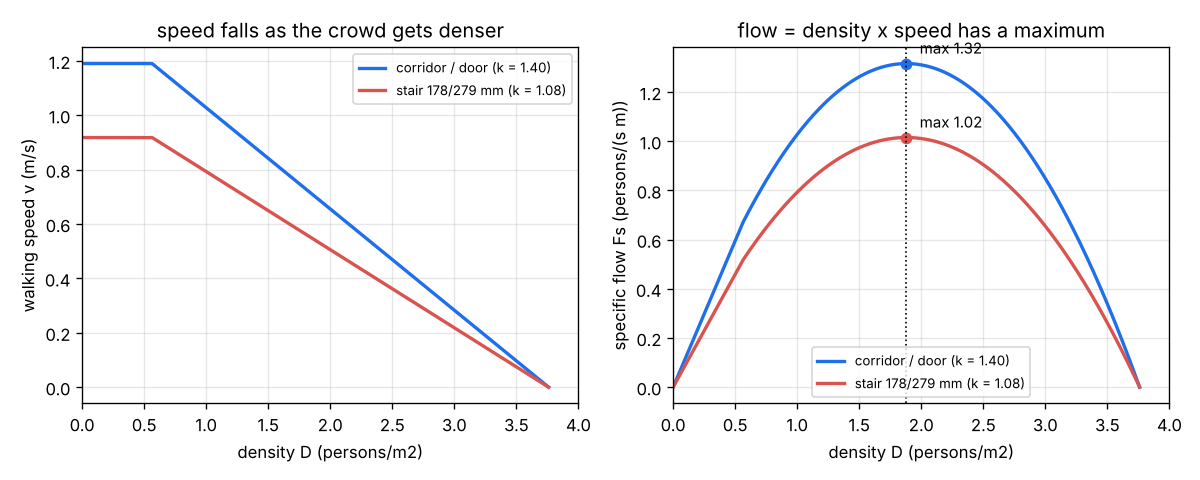
\includegraphics[width=0.85\linewidth]{figures/s02_fundamental_diagram.png}\\\small Speed against density (left) and specific flow against density (right) for level ground and a stair; the flow has a maximum at 1.88 persons/m2.\end{center}

\subsection*{E. Worked example}
A 2.0 m wide corridor carries a crowd at a density of 1.0 persons/m2 towards a 1.2 m door. Find the walking speed, the flow arriving, the largest flow the door can pass, and how fast the queue grows.
\begin{enumerate}[nosep]
\item Speed: v = 1.40 x (1 - 0.266 x 1.0) = 1.40 x 0.734 = 1.028 m/s.
\item Specific flow in the corridor: Fs = D v = 1.0 x 1.028 = 1.028 persons/(s m).
\item Effective corridor width: 2.0 - 2 x 0.20 = 1.6 m, so the flow arriving is 1.028 x 1.6 = 1.644 persons/s.
\item Door: We = 1.2 - 2 x 0.15 = 0.9 m and Fs\_max = 1.40 / (4 x 0.266) = 1.316, so it passes at most 1.316 x 0.9 = 1.184 persons/s.
\item Conservation: 1.644 arrive but only 1.184 leave, so the queue grows at 1.644 - 1.184 = 0.460 persons/s, about 28 people per minute.
\end{enumerate}
\textbf{Answer.} v = 1.03 m/s, 1.64 persons/s arrive, the door passes 1.18 persons/s and a queue grows at 0.46 persons/s. A door with We = 1.644 / 1.316 = 1.25 m (clear width 1.55 m) would avoid it.

\subsection*{F. Questions}
\begin{enumerate}[nosep]
\item \textbf{Conceptual.} Why does pushing into a crowded doorway reduce the number of people who get through each second?
\item \textbf{Numerical.} Find the walking speed and the specific flow at D = 2.5 persons/m2 on level ground, and on a stair with k = 1.08 m/s. Compare with the maxima.
\item \textbf{Graph and simulation interpretation.} On the flow curve, the same specific flow of 1.0 persons/(s m) appears at two densities. Find both and explain which one a corridor has before and after a bottleneck.
\item \textbf{Design and optimisation challenge.} Design: a 2.4 m corridor will carry a crowd at 1.2 persons/m2 into a stair of steps 178/279 mm. What is the narrowest clear stair width that avoids a queue at the top of the stair? Compare with the door width that would be enough on level ground.
\end{enumerate}

\section{Session 3: Simulate a building evacuation and plan it safely}

\subsection*{A. Real-world problem}
A college block has a ground floor and three upper floors with 120 people on each, 480 in all. Everyone above the ground floor must use the stairs. How long does the block take to empty, where do the queues form, and how many stairs of what width are needed so that everyone is out well before smoke makes the stairs unsafe, even if smoke blocks one stair? (A simplified teaching model, not a design tool.)

\subsection*{B. Concept and theory}
Every door and every stair flight (one storey of stair) is a \textbf{link} with a \textbf{capacity} C (the largest flow, Fs\_max x We from Session 2), a \textbf{travel time} tau (length divided by the free walking speed) and a \textbf{next} link. Each link has a queue at its entrance. The simulation moves a clock forward in steps of dt = 0.5 s. In each step at most C dt people leave the queue of a link; they walk for tau seconds and then join the queue of the next link, or reach the outside. Upper-floor people pass through their stair door onto the stair; the people coming down from above join the same queue, so the floors \textbf{merge}. Ground-floor people go straight to the final exit, which also takes everyone off the stair. A simulation is only useful once it is \textbf{validated}: (1) one room with one door must give the Session 1 formula; (2) no person is lost or created; (3) everyone above the ground floor must pass the lowest stair flight, so the evacuation cannot be faster than t\_bound = t\_pre + L / v + (floors x n) / C\_stair + tau\_stair; (4) a smaller time step must give nearly the same answer. Safety is judged by two times. \textbf{RSET} (required safe escape time) = detection + pre-movement + movement. \textbf{ASET} (available safe escape time) is how long until smoke or heat make the route untenable; it comes from a fire model and is given here. A plan is acceptable here when 1.5 x RSET $\le$ ASET, both with all stairs open and with one stair blocked.

\begin{itemize}[nosep]
\item C: capacity of a link: Fs\_max x We (persons/s)
\item tau: travel time through a link (s)
\item dt: simulation time step (s)
\item n: people per floor (persons)
\item t\_evac: time when the last person is outside (s)
\item t\_detect: time from the start of the fire to the alarm (s)
\item RSET, ASET: required and available safe escape time (s)
\end{itemize}

\begin{equation*}
C = F_{s,\max}\,W_e = \frac{k}{4a}\,(W - 0.30\ \mathrm{m}),\qquad \tau = \frac{L}{0.85\,k}
\end{equation*}

\begin{equation*}
\text{each step: served} = \min(Q,\ C\,dt),\quad Q \leftarrow Q - \text{served} + \text{arrivals from upstream}
\end{equation*}

\begin{equation*}
t_{\mathrm{evac}} \ge t_{\mathrm{bound}} = t_{\mathrm{pre}} + \frac{L}{v} + \frac{n_{\mathrm{floors}}\,n}{C_{\mathrm{stair}}} + \tau_{\mathrm{stair}}
\end{equation*}

\begin{equation*}
\mathrm{RSET} = t_{\mathrm{detect}} + t_{\mathrm{evac}},\qquad \text{safe if } 1.5 \times \mathrm{RSET} \le \mathrm{ASET}
\end{equation*}

\begin{center}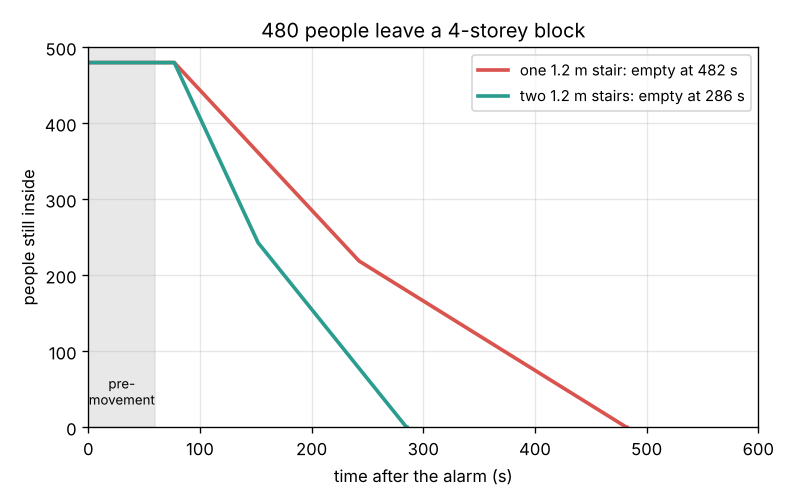
\includegraphics[width=0.85\linewidth]{figures/s03_building_emptying.png}\\\small 480 people leave a four-storey block with one or two 1.2 m stairs.\end{center}

\subsection*{E. Worked example}
The block has 3 upper floors and a ground floor, 120 people each, one stair 1.2 m wide (178/279 mm steps, 9 m per flight), 1.2 m stair doors and a 1.5 m final exit. Pre-movement 60 s, corridor 20 m. Estimate the evacuation time by hand, compare with the simulation, and check the plan against ASET = 900 s.
\begin{enumerate}[nosep]
\item Stair capacity: We = 1.2 - 0.3 = 0.9 m, Fs\_max = 1.08 / (4 x 0.266) = 1.015, so C = 0.914 persons/s. The stair door (1.184 persons/s) and the exit (1.579 persons/s) are wider in flow, so the stair is the bottleneck.
\item First arrival at the stair: 60 + 20 / 1.19 = 76.8 s. Time for the 360 upper-floor people to pass the lowest flight: 360 / 0.914 = 394.1 s. Last person's walk down the flight: 9 / 0.918 = 9.8 s.
\item Hand bound: 76.8 + 394.1 + 9.8 = 480.7 s. The simulation gives 482.5 s, just above the bound (the stair is idle for a few seconds at the start while the first people walk down).
\item RSET = 30 + 482.5 = 512.5 s, and 1.5 x 512.5 = 769 s, below 900 s: safe with one 1.2 m stair, but no reserve if it is blocked.
\item Plan with two stairs: both open, RSET = 316 s; one blocked, everyone uses the other: RSET = 512 s, still safe. Two 1.0 m stairs fail the blocked case (RSET 625 s, 1.5 x 625 = 938 s > 900 s).
\end{enumerate}
\textbf{Answer.} About 481 s by hand, 482.5 s simulated. Plan: two 1.2 m stairs (RSET 316 s, or 512 s with one blocked).

\subsection*{F. Questions}
\begin{enumerate}[nosep]
\item \textbf{Conceptual.} With one stair, why do the people on the top floor not wait the longest, even though they are farthest from the exit?
\item \textbf{Numerical.} For the same block, find the hand bound with one 1.5 m stair, and the RSET. Is it safe for ASET = 900 s with the factor 1.5?
\item \textbf{Graph and simulation interpretation.} In the queue figure, the stair-door queue on floor 2 stays flat at about 110 people from 90 s to 220 s and then falls in a straight line. Explain the flat part and the slope.
\item \textbf{Design and optimisation challenge.} Design: the four-storey block (3 upper floors, 120 each) has ASET = 900 s. Using the safety factor 1.5, choose the number of stairs and the narrowest width (1.0, 1.2, 1.5 or 2.0 m) that is safe even with one stair blocked. Then say why a single 2.0 m stair, which is also "safe", is a poor plan.
\end{enumerate}

\section{Real-world mini-project}
\textbf{Plan the stairs of a student hostel.} A six-storey student hostel has a ground floor and five upper floors with 150 residents on each (900 in all). Use \texttt{stair\_rset} and \texttt{plan\_stairs} from Session 3 with the default corridor, stair flight and pre-movement values, a detection time of 30 s and an illustrative ASET of 1200 s with a safety factor of 1.5. The warden asks: how many stairs, how wide, and is the plan still safe at night if smoke fills one stair? These limits are illustrative numbers, not code requirements.

\section{The path ahead}
\begin{enumerate}[nosep]
\item \textbf{Session 4: People are not all the same.} Pre-movement times (for example lognormal) and walking speeds drawn per person or per group, released into the Session 3 network, and a Monte Carlo of 500 runs that reports the mean and the 95th-percentile evacuation time.
\item \textbf{Session 5: Draw the floor plan.} A reader for a small text file of nodes and links (width, length, kind), shortest-route exit choice (Dijkstra), and the Session 3 simulation running on that graph.
\item \textbf{Session 6: Counterflow and merging rules.} A lane of the stair reserved for counterflow (a reduced effective width) and three merging rules on landings: first come, floor priority, and taking turns.
\item \textbf{Session 7: People as agents.} A 2D simulation of individuals leaving a room through one door, with a few hundred agents and simple time stepping.
\item \textbf{Session 8: Smoke and ASET.} A two-zone smoke-filling model that gives the time until the smoke layer reaches 2 m (ASET), and a walking speed that falls inside smoke.
\end{enumerate}

\section{Answers and hints}

\subsection*{Session 1}
\begin{enumerate}[nosep]
\item \textbf{Conceptual.} Hint: Which of the three parts of t\_evac depends on the number of doors? Solution: Only the queue time N / F depends on the doors. Doubling the doors doubles F and halves the queue time (205 s to 103 s), but the pre-movement time (60 s) and the walk to the door (17 s) stay the same. So the total goes from 282 s to 179 s, a cut of 37 percent, not 50 percent. To shorten the evacuation further you must also shorten the pre-movement time, for example with a clear alarm and trained wardens.
\item \textbf{Numerical.} Hint: We = 1.0 - 0.3; then add t\_pre, L / v and N / F. Solution: We = 0.7 m, so F = 1.3 x 0.7 = 0.91 persons/s. Walking: 12 / 1.2 = 10 s. Queue: 150 / 0.91 = 164.8 s (persons divided by persons per second gives seconds). Total: 30 + 10 + 164.8 = 204.8 s, about 3.4 minutes. Reasonable: the queue dominates because the door is narrow.
\item \textbf{Graph and simulation interpretation.} Hint: Compare the effective widths, not the clear widths. Solution: The effective widths are 0.9 m and 2.1 m, a factor 2.33, because the two 0.15 m edge strips are lost only once. Queue times: 240 / (1.3 x 0.9) = 205.1 s and 240 / (1.3 x 2.1) = 87.9 s. Totals: 281.8 s and 164.6 s. The total falls by less than half, again because 76.7 s of waiting and walking stays.
\item \textbf{Design and optimisation challenge.} Hint: The queue may last at most 240 - 76.7 = 163.3 s, so F must be at least 300 / 163.3 persons/s. Solution: Needed: F = 300 / 163.3 = 1.84 persons/s, so total effective width at least 1.84 / 1.3 = 1.41 m. Two 1.0 m doors: We = 1.4 m, t = 76.7 + 300 / 1.82 = 241.5 s: just misses. Two 1.2 m doors: We = 1.8 m, t = 76.7 + 128.2 = 204.9 s: meets it. One 1.8 m door: We = 1.5 m, t = 76.7 + 153.8 = 230.5 s: meets it on paper. Choose two 1.2 m doors at opposite ends: if a fire blocks one door, the other still works, and a single door gives no such choice. Building codes ask for at least two exits from large rooms for exactly this reason.
\end{enumerate}

\subsection*{Session 2}
\begin{enumerate}[nosep]
\item \textbf{Conceptual.} Hint: Look at the right half of the flow curve, above 1.88 persons/m2. Solution: Flow is density times speed. Up to 1.88 persons/m2 more people per square metre wins: the flow rises. Above it the speed falls faster than the density rises, so the product falls; at 3.8 persons/m2 nobody moves. Pushing raises the density above the best value, so fewer people pass per second, and it adds the danger of falls and crushing. Calm, steady movement at a moderate density gives the most flow.
\item \textbf{Numerical.} Hint: 1 - 0.266 x 2.5 = 0.335. Solution: Level: v = 1.40 x 0.335 = 0.469 m/s, Fs = 2.5 x 0.469 = 1.17 persons/(s m), below the maximum 1.32. Stair: v = 1.08 x 0.335 = 0.362 m/s, Fs = 0.905 persons/(s m), below its maximum 1.02. Both are on the falling, congested side of the curve.
\item \textbf{Graph and simulation interpretation.} Hint: Solve 1.40 D (1 - 0.266 D) = 1.0, a quadratic in D. Solution: 0.3724 D\textasciicircum{}2 - 1.40 D + 1.0 = 0 gives D = (1.40 -/+ sqrt(1.96 - 1.4896)) / 0.7448 = (1.40 -/+ 0.686) / 0.7448, so D = 0.96 or 2.80 persons/m2. Upstream of a bottleneck, in the queue, the crowd is dense and slow (2.80, the congested side). After it, the same flow spreads out and moves freely (0.96, the free side). This is the same as traffic before and after a narrowing of a road.
\item \textbf{Design and optimisation challenge.} Hint: Flow in = Fs(1.2) x (2.4 - 0.4). The stair can take at most 1.015 x We. Solution: v = 1.40 x (1 - 0.319) = 0.953 m/s, Fs = 1.144, We = 2.0 m, so 2.29 persons/s arrive. Stair: We needed = 2.29 / 1.015 = 2.25 m, clear width 2.25 + 0.30 = 2.55 m. A level door would need 2.29 / 1.316 = 1.74 m effective, 2.04 m clear. The stair needs about 0.5 m more because people are slower on steps. Trade-off: a wide stair costs floor area on every storey; designers often accept a short queue at the stair door instead, as long as the total evacuation time is safe (Session 3).
\end{enumerate}

\subsection*{Session 3}
\begin{enumerate}[nosep]
\item \textbf{Conceptual.} Hint: Where do all upper-floor people have to pass, and who reaches it first? Solution: Nobody comes down to the top landing from above, so its queue drains at the full stair capacity from the start and is empty at 208 s. Every lower landing also receives people from the floors above, as fast as the flight below takes people away, so its queue stays flat until the floors above have emptied. The floor-1 landing, at the top of the lowest flight that everyone above the ground floor must pass, is the last to clear (472 s). In this simple model, without priority rules, people nearest the bottom wait the longest, and the total time is set by the bottleneck, not by the height. Real crowds merge differently (often close to taking turns), which changes who waits but not the total time through the bottleneck.
\item \textbf{Numerical.} Hint: C = 1.015 x 1.2 persons/s. Solution: C = 1.015 x 1.2 = 1.218 persons/s. Bound: 76.8 + 360 / 1.218 + 9.8 = 76.8 + 295.6 + 9.8 = 382.2 s (simulation: 384 s with 1.5 m doors and a 1.8 m exit). RSET = 30 + 384 = 414 s, 1.5 x 414 = 621 s < 900 s: safe. Check: a wider stair gives a smaller time, and the queue part fell by the ratio of effective widths 0.9 / 1.2.
\item \textbf{Graph and simulation interpretation.} Hint: Who is using the stair while floor 2 waits? Solution: The landing queue holds both floor-2 people and floor-3 people who have walked down to it. While floor 3 is emptying, people arrive from above at 0.91 persons/s and the flight below takes 0.91 persons/s away, so the queue stays constant. When floor 3 has passed (about 210 s), nobody arrives from above and the queue drains at the stair capacity, about 0.91 persons/s (110 people in about 120 s), the straight line, until 340 s. The short drop from 120 to 111 at the start is the few seconds before the first floor-3 people arrive. Merging rules (who goes first on a landing) are a known weakness of simple models.
\item \textbf{Design and optimisation challenge.} Hint: Use plan\_stairs(900) and compare stair\_rset(1, w) for each width. Solution: RSET must be at most 600 s. Two 1.0 m stairs: one blocked gives 625 s: fails. Two 1.2 m stairs: 316 s both open, 512 s one blocked: safe. So two 1.2 m stairs. A single 2.0 m stair has RSET 327 s, but if smoke enters it there is no way out at all; fire codes require at least two independent escape routes from upper floors for that reason. Trade-off: two stairs cost more floor area, but they give a route that survives one failure.
\end{enumerate}

\section{How to join}
Read \texttt{CONTRIBUTING.md} in the repository, then pick an issue labelled \texttt{good first issue}. Repository: \url{https://github.com/KrunalPanchal1995/pan-iit-oss/tree/main/openevacuation}

\end{document}
